
\documentclass[11pt, aspectratio=169]{beamer}

\usepackage[utf8]{inputenc}
\usepackage{tikz}
\usepackage[english]{babel}
\usepackage{svg}
\usepackage{eurosym}
\usepackage{subfig}
\usepackage{pgfgantt}
\usepackage[export]{adjustbox}
%\usepackage[shortlabels]{enumitem}
\usepackage[font=scriptsize,justification=centering]{caption}
\usepackage{movie15}

%----------------------------------------------------------------------------------------
%	TITLE PAGE INFORMATION.
%----------------------------------------------------------------------------------------
\author{A. M\"{o}slinger, K. Steele, D. Talavera, N. Ulfvarson, and E.F.M. Weterings}
\title{InfraRed Imaging of astronomical targets with a Stabilised Camera}
\subtitle{IRISC}
\institute{DLR MORABA, Oberpfaffenhofen} 
\date{11-15 February 2019}
%\subject{} 

%----------------------------------------------------------------------------------------
%	SETUP LAYOUT.
%----------------------------------------------------------------------------------------
\usepackage{theme/beamerthemeWarsawLTU}
%\usetheme{Warsaw}


\begin{document}
%----------------------------------------------------------------------------------------
%	TITLE PAGE.
%----------------------------------------------------------------------------------------

{\setbeamertemplate{logo}{}
\begin{frame}
\titlepage
\begin{tikzpicture}[remember picture,overlay]
    \node[xshift=13cm,yshift=-1.025\textheight,anchor=north west] at (current page.north west){%
    
\includegraphics[width=2cm]{theme/LTU_logo.jpg}};
\end{tikzpicture}
\end{frame}
}

%----------------------------------------------------------------------------------------
%	TABLE OF CONTENTS.
%----------------------------------------------------------------------------------------
\begin{frame}[t]{Table of Contents}
\vspace{-0.3cm}
    \begin{columns}[t]
        \begin{column}{.5\textwidth}
            \tableofcontents[sections={1-2}]
        \end{column}
        \begin{column}{.5\textwidth}
            \tableofcontents[sections={3-5}]
            \vspace{-.2cm}
            \tableofcontents[sections=6,hidesubsections]
        \end{column}
    \end{columns}
\end{frame}


%----------------------------------------------------------------------------------------
%	INTRODUCTION.
%----------------------------------------------------------------------------------------
\section{IRISC: In a Nutshell}
\begin{frame}[c]{In a Nutshell}
    \centering
    \huge Our vision is to make astronomical research more accessible by developing a stabilised balloon-borne telescope
\end{frame}


%----------------------------------------------------------------------------------------
%	SYSTEM.
%----------------------------------------------------------------------------------------
\section{System}

%----------------------------------------------------------------------------------------
%	SCIENCE.
%----------------------------------------------------------------------------------------
\section{Science}

%----------------------------------------------------------------------------------------
%	PROJECT MANAGEMENT.
%----------------------------------------------------------------------------------------
\section{Project Management}

%----------------------------------------------------------------------------------------
%	SUMMARY.
%----------------------------------------------------------------------------------------
\section{Summary}

%----------------------------------------------------------------------------------------
%	QUESTIONS.
%----------------------------------------------------------------------------------------
\section{Questions}

%\begin{frame}[plain]{}
%%    \label{slide:questions}
%%    \centering
%%    \vspace{-0.71cm}
%%    \begin{figure}
%%    \hspace*{-1.1cm}
%%    	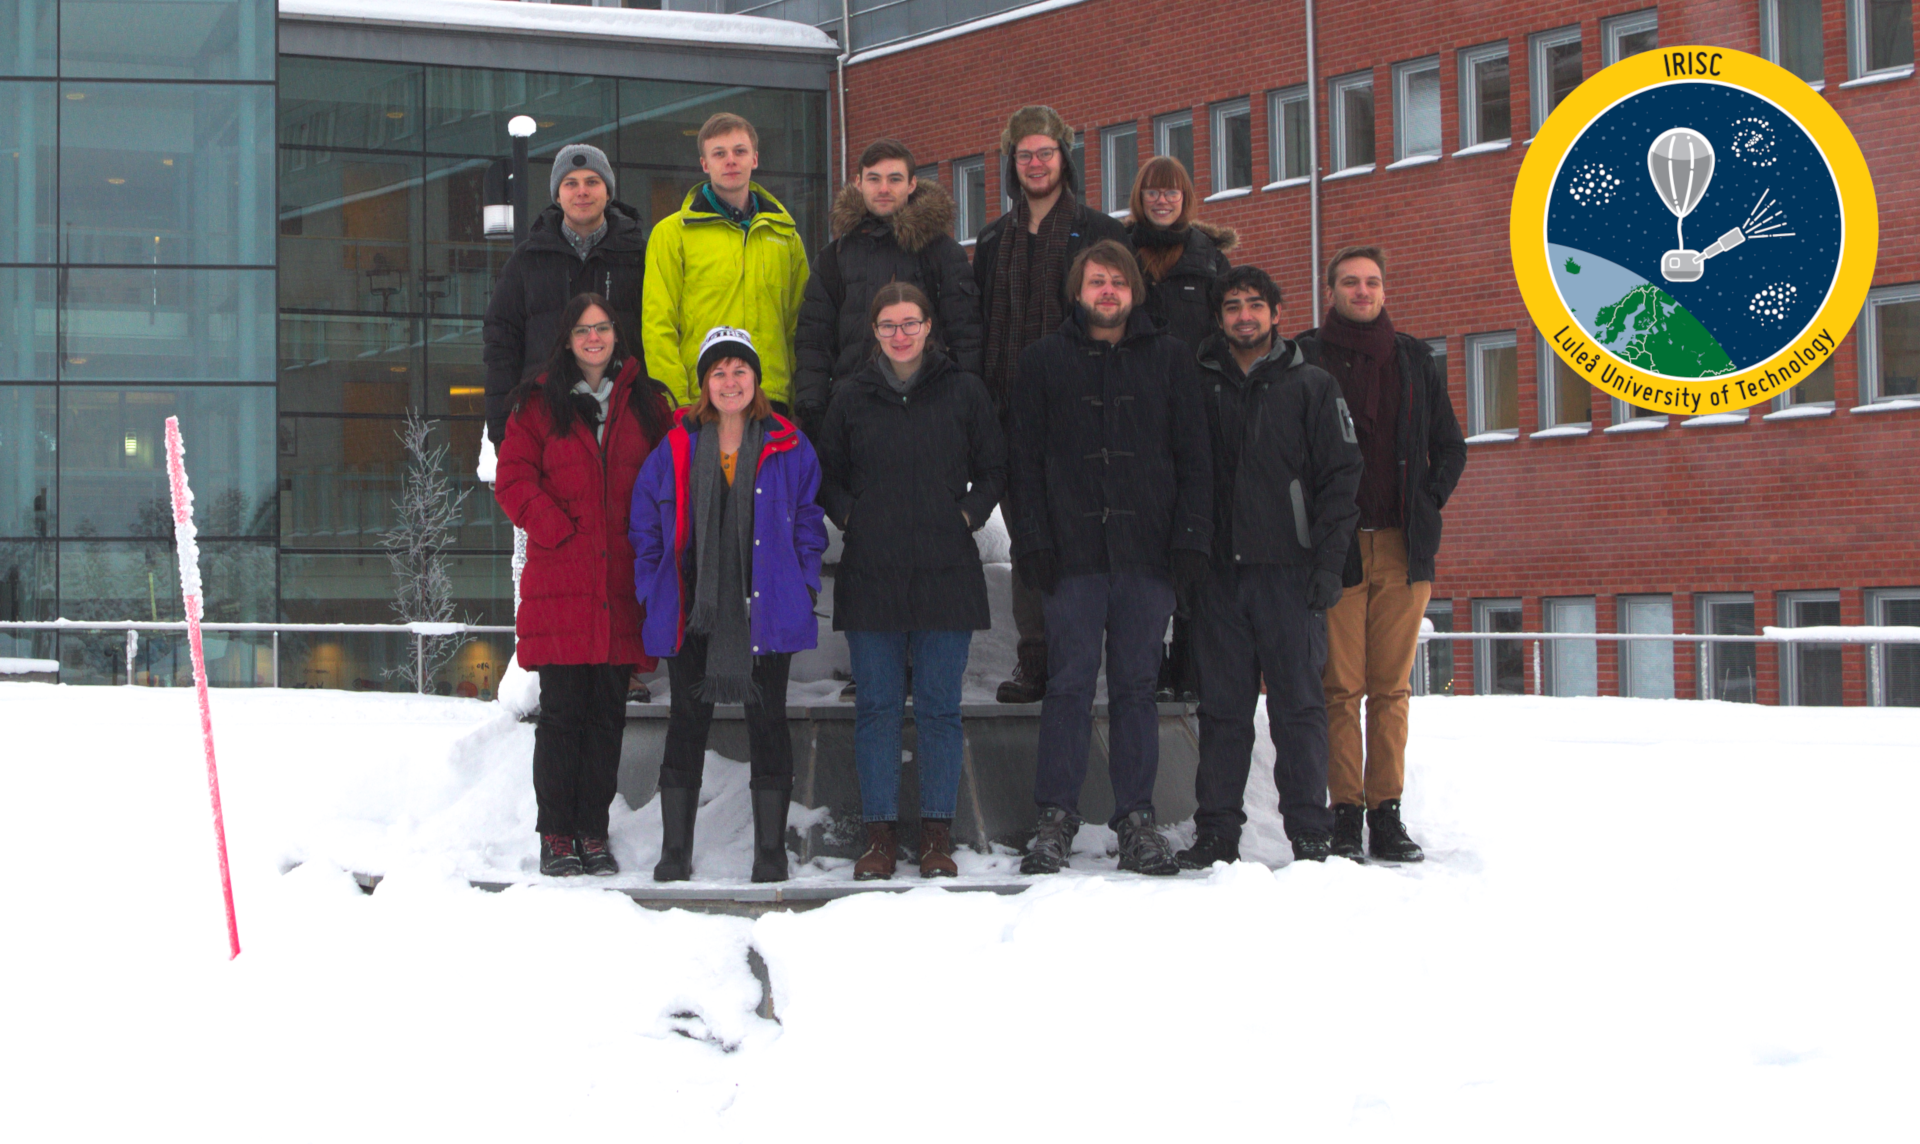
\includegraphics[width=1.15\textwidth]{figures/images/teamphoto.png}
%%    \end{figure}
%	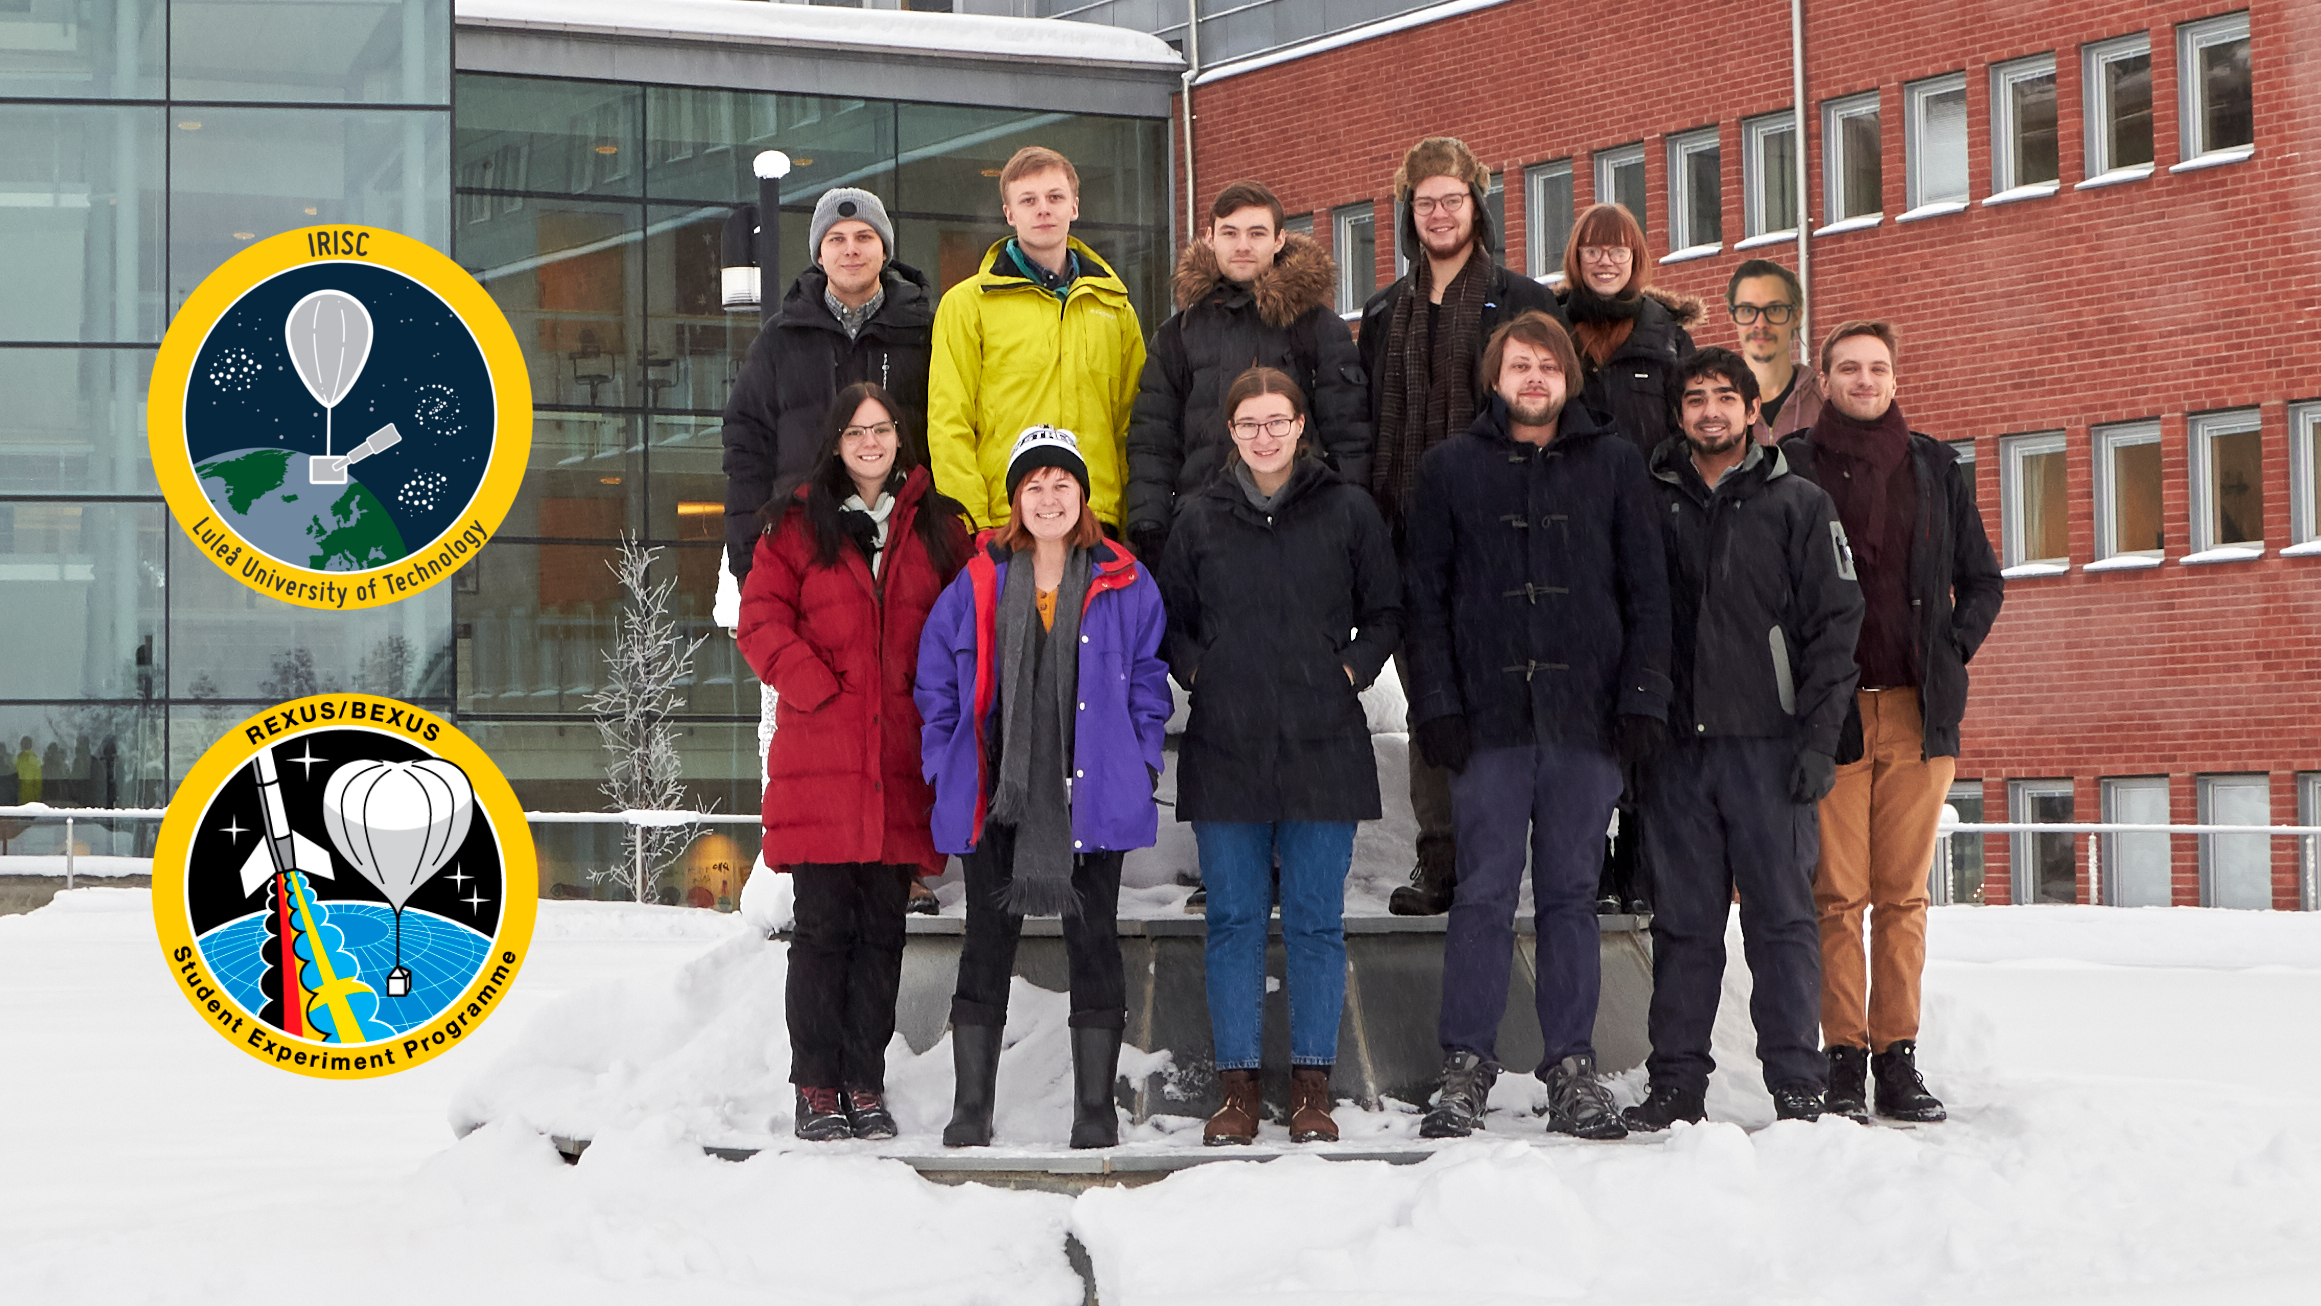
\includegraphics[width=\paperwidth]{figures/images/IRISC_Team_001_16_9+logo.jpg}
%\end{frame}
{
\usebackgroundtemplate{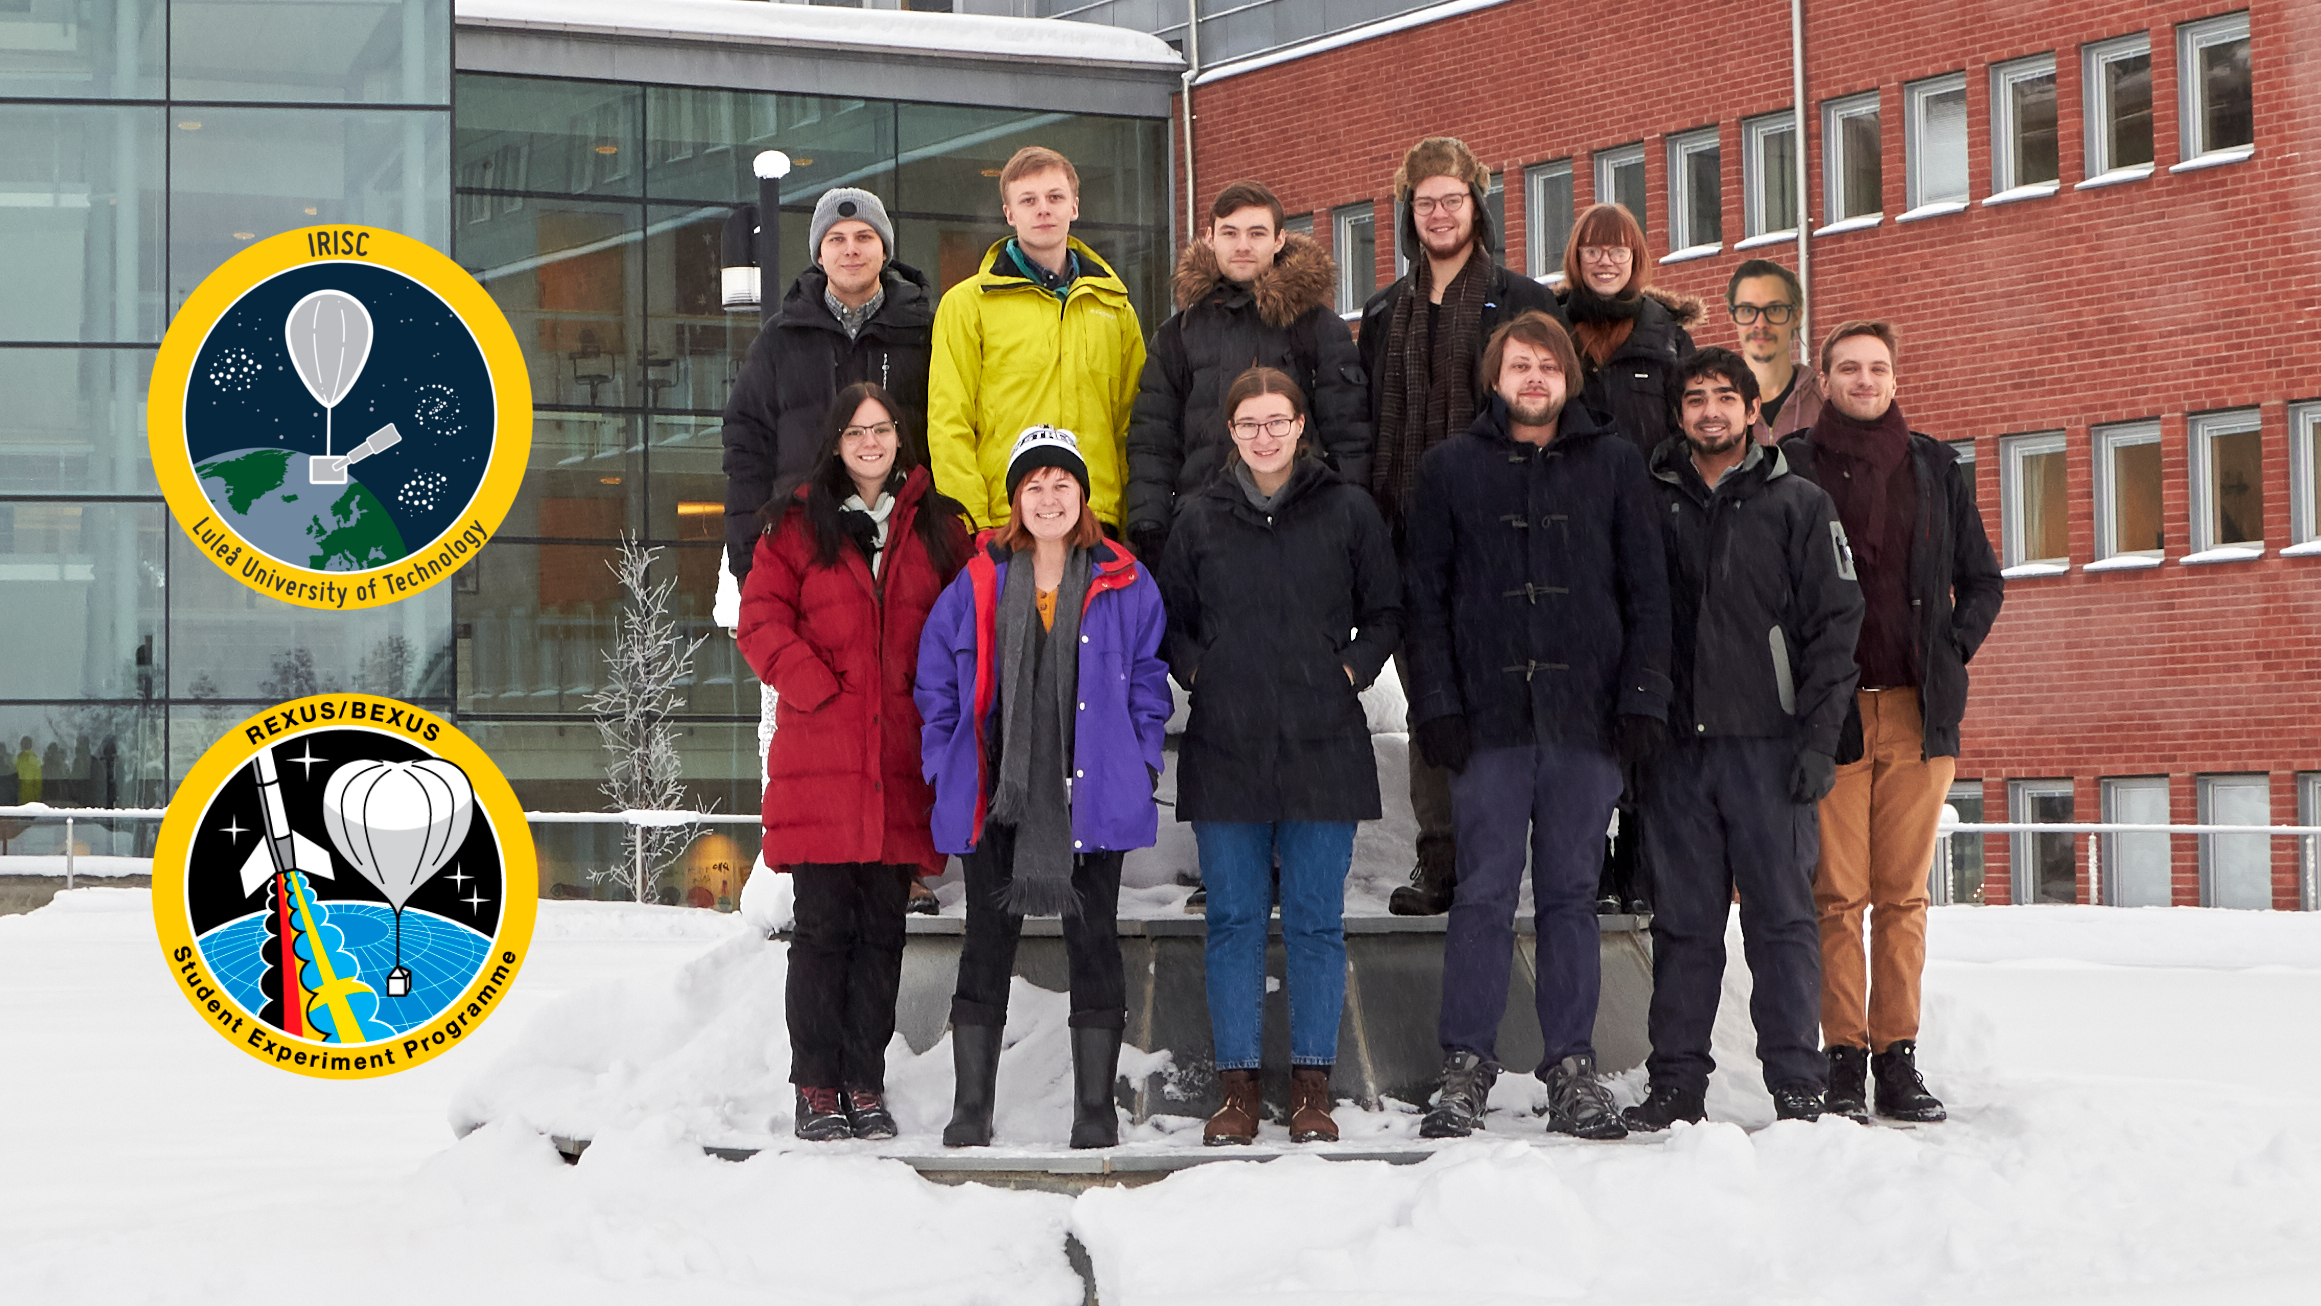
\includegraphics[width=\paperwidth]{figures/images/IRISC_Team_001_16_9+logo.jpg}}
\begin{frame}[plain]
%\label{slide:questions}
\end{frame}

}
%----------------------------------------------------------------------------------------
%	BACKUP SLIDES. 				EVERYONE!!!
%----------------------------------------------------------------------------------------

\end{document}
